\documentclass{article}
\usepackage{tikz}
\usetikzlibrary{calc}
\begin{document}
	\begin{figure}
		\begin{center}
			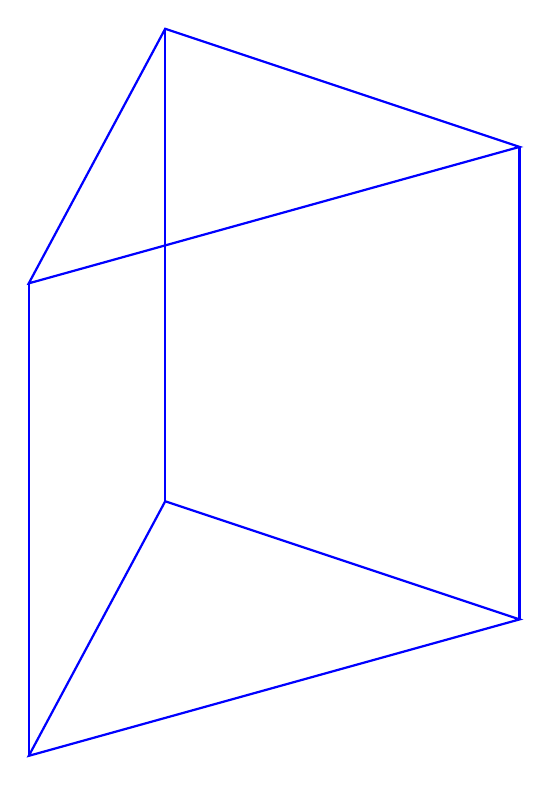
\begin{tikzpicture}[scale = 1.5,fill,blue,thick]
				\coordinate (A) at (3,0,0);
				\coordinate (B) at (0,1,0);
				\coordinate (C) at (0,0,3);
				\coordinate (H) at (0,4,0);
				
				\draw (A) -- (B) -- (C) -- cycle;
				\draw ($(A)+(H)$) -- ($(B)+(H)$) -- ($(C)+(H)$) -- cycle;
				\draw (A) -- ($(A)+(H)$) (B) -- ($(B)+(H)$) (C) -- ($(C)+(H)$);
			\end{tikzpicture}
			\caption{3D Drawing}
		\end{center}
	\end{figure}
\end{document}